\documentclass[svgnames,dvipsnames,hyperref={bookmarks=false},usepdftitle=false]{beamer}
\usetheme{curryon}

\title{To Macros and Beyond!}
\subtitle{How macros changed Scala, and what's coming next}
\author{Eugene Burmako}
\institute{
\includegraphics[height=2cm]{epfl.png}}
\date{19 July 2016}
\hypersetup{pdfauthor={Eugene Burmako},pdftitle={What I Learned From Inventing Scala Macros}}

\begin{document}

\titleframe

\begin{frame}[fragile]{Who am I?}
\begin{semiverbatim}
\text{\color{gray}{\$ git config --get remote.origin.url}}
https://github.com/scala/scala

\text{\color{gray}{\$ git shortlog --author=Burmako -sn --no-merges | awk ...}}
763 commits

\text{\color{gray}{\$ git log --author=Burmako --numstat | awk ...}}
146492 lines added
96869 lines removed
\end{semiverbatim}
\end{frame}

\begin{frame}{In today's talk}
\begin{itemize}
\item Battle-tested design that marries macros and types
\item The best and the worst things about Scala macros
\item What's coming next in future versions of the language
\end{itemize}
\end{frame}

\sectionframe{A whirlwind tour}

\begin{frame}{Inception}

\includegraphics[height=1.5cm]{nemerle.png}
\begin{itemize}
\item Scala macros started as my first semester project at EPFL
\item I just joined the PhD program and knew close to nothing about Scala
\item But I really liked macros in Nemerle
\end{itemize}
\end{frame}

\begin{frame}[fragile]
\frametitle{Use case}

\includegraphics[height=1.5cm]{slick.png}
\begin{itemize}
\item Database query and access library for Scala
\item Joint EPFL + Lightbend project, kicked off in Sep 2011
\item Needed some form of language-integrated queries
\end{itemize}
\end{frame}

\begin{frame}[fragile]
\frametitle{Use case}

\begin{semiverbatim}
val users: Table[User] = ...
users.map(\alert{u => u.name})

                          \arrowdown

val users: Table[User] = ...
new Table(Map(users, \alert{Ref("name", classOf[String])}))

\end{semiverbatim}

\begin{itemize}
\item Allow users to write queries in normal Scala
\item Somehow transform these queries into a custom representation
\item Compile the representation to SQL, etc
\end{itemize}
\end{frame}

\begin{frame}[fragile]
\frametitle{Idea \#1}

\begin{semiverbatim}
class Table[T](val query: Query[T]) \{
  def map[U](fn: \alert{scala.reflect.Expr[T => U]}) = ...
\}

val users: Table[User] = ...
users.map(\alert{u => u.name})

\end{semiverbatim}

\begin{itemize}
\item Have the compiler magically convert \texttt{T} to \texttt{Expr[T]}
\item Expression trees can then be analyzed at runtime
\item This is how it's done in C\# and F\#
\end{itemize}
\end{frame}

\begin{frame}[fragile]
\frametitle{Idea \#2}

\begin{semiverbatim}
object Macros \{
  def map(fn: \alert{compiler.Tree}) = ...
\}

val users: Table[User] = ...
users.map(\alert{u => u.name})

\end{semiverbatim}

\begin{itemize}
\item Have the compiler run user-defined code during compilation
\item During compilation, code is represented with trees anyway
\item Compile-time processing brings a number of additional benefits
\end{itemize}
\end{frame}

\begin{frame}[fragile, t]
\frametitle{Implementation}

\begin{semiverbatim}
class Table[T](val query: Query[T]) \{
  \alert<1>{def map[U](fn: T => U): Table[U] = \alert<2>{macro \only<1>{...}}\alert<2>{\only<2->{Macros.map}}}
\}

\only<2->{object Macros \{
  \alert<2>{def map(c: Context)(fn: c.Tree): c.Tree} = \only<2>{...}\only<3->{\{
    val subquery: c.Tree = translate(fn)
    \alert<3>{q"new Table(Map(\$\{}c.prefix\alert<3>{\}, \$}subquery\alert<3>{))"}
  \}}
\}}

\end{semiverbatim}

\begin{itemize}
\only<1->{\item Macros look like normal Scala methods}
\only<2->{\item Implementations are written against a dedicated reflection API}
\only<3->{\item Reflection API includes quasiquotes to perform AST manipulations}
\end{itemize}
\end{frame}

\begin{frame}[fragile]
\frametitle{Usage}

\begin{semiverbatim}
val users: Table[User] = ...
\alert{users.map(u => u.name)}

                          \arrowdown

val users: Table[User] = ...
\alert{new Table(Map(users, Ref("name", classOf[String])))}

\end{semiverbatim}

\begin{itemize}
\item When the user writes \texttt{Table.map}, the compiler calls \texttt{Macros.map}
\item \texttt{Macros.map} expands in a domain-specific fashion
\item Compiler replaces the call to \texttt{Table.map} with the macro expansion
\end{itemize}
\end{frame}

\begin{frame}[fragile]
\frametitle{Language-integrated queries via macros}
\begin{semiverbatim}
class Table[T](val query: Query[T]) \{
  def map[U](fn: T => U): Table[U] = macro Macros.map
\}

object Macros \{
  def map(c: Context)(fn: c.Tree): c.Tree = \{
    val subquery: c.Tree = translate(fn)
    q"new Table(Map(\$\{c.prefix\}, \$subquery))"
  \}
\}
\end{semiverbatim}
\end{frame}

\sectionframe{The best thing about Scala macros}

\begin{frame}{The best thing about Scala macros}
\begin{itemize}
\item After the public release, macros have spread like wildfire
\item E.g. all libraries in Lightbend stack have used or are using our stuff
\item Why did this happen?
\end{itemize}
\end{frame}

\begin{frame}[fragile]
\frametitle{The best thing about Scala macros}

\begin{itemize}
\item Macros piggyback on a familiar concept of a typed method call
\item This allows existing code to easily absorb new meanings
\item A lot of language features become transparently enriched
\end{itemize}
\end{frame}

\begin{frame}[fragile]
\frametitle{Enriched interpolation}

\begin{semiverbatim}
scala> val x = "42"
x: String = 42

scala> "%d".format(x)
j.u.IllegalFormatConversionException: d != java.lang.String
  at j.u.Formatter\$FormatSpecifier.failConversion...
\only<2>{
scala> \alert{f"}\$x\%d\alert{"}
error: type mismatch;
 found   : String
 required: Int
}
\end{semiverbatim}

\begin{itemize}
\item Scala's type system can't typecheck format strings
\only<2>{\item With macros, this stops being an issue}
\only<2>{\item By integrating with other features, macros solve the problem at hand}
\end{itemize}
\end{frame}

\begin{frame}[fragile]{String interpolation}
\begin{semiverbatim}
scala> val world = "world"
world: String = "world"

scala> s"hello, \$world!"
res0: String = "hello, world!"

\only<2->{scala> desugar(\text{\color{red}{s}}"\alert{hello, }\text{\color{teal}{\$world}}\alert{!}")}
\only<2->{res1: Tree = StringContext(\alert{"hello, "}, \alert{"!"}).\text{\color{red}{s}}(\text{\color{teal}{world}})}

\only<3->{scala> // string interpolation also works in patterns
       // check out our docs for more details}
\end{semiverbatim}
\end{frame}

\begin{frame}[fragile]{Extension methods}
\begin{semiverbatim}
scala> f"hello, \$world!"
error: value f is not a member of StringContext

\only<2->{scala> implicit class AnyNameYouWant(\alert<4>{ctx: StringContext}) \{}
\only<2->{     |   def \text{\color<4>{red}{f}}(\text{\color<4>{teal}{args: Any*}}): String = ...}
\only<2->{     | \}}
\only<2->{defined class AnyNameYouWant}

\only<3->{scala> \text{\color<4>{red}{f}}"\alert<4>{hello, }\text{\color<4>{teal}{\$world}}\alert<4>{!}"}
\only<3->{res2: String = ...}
\end{semiverbatim}
\end{frame}

\begin{frame}[fragile]
\frametitle{Enriched interpolation}

\begin{semiverbatim}
implicit class Formatter(c: StringContext) \{
  \alert{def f(args: Any*): String = macro ...}
\}

val x = "42"
\alert{f"}\$x\%d\alert{"} // rewritten into: StringContext("", "%d").\alert{f(}x\alert{)}

                          \arrowdown

\{
  val arg\$1: Int = x \alert{// doesn't compile}
  "%d".format(arg\$1)
\}

\end{semiverbatim}

\begin{itemize}
\item \texttt{f} is a macro that inserts type ascriptions in strategic places
\item Macros enrich string interpolation with new powers
\end{itemize}
\end{frame}

\begin{frame}[fragile]
\frametitle{Other examples}
More examples of enriching existing language features with macros:
\begin{itemize}
\item Quasiquotes
\item \texttt{async}/\texttt{await}
\item Deep embedding of DSLs
\item Typeclass derivation
\item Fast automatic serialization
\item Type providers
\end{itemize}
\end{frame}

\sectionframe{The most complicated thing about Scala macros}

\begin{frame}{Implementation effort}
\begin{itemize}
\item 750-1000 commits
\item 150-250kloc accumulated changes
\item 50kloc added
\end{itemize}
\end{frame}

\begin{frame}{Implementation breakdown}
In increasing order of time spent:
\begin{itemize}
\item<1-> Macro engine (2kloc, several key findings)
\item<2-> Discussions with the language committee (hundreds of hours)
\item<3-> Community building (dozens of talks, thousands of emails)
\item<4-> \alert{Fleshing out scala.reflect (9kloc, 12kloc docs, several rewrites)}
\end{itemize}
\end{frame}

\sectionframe{The worst thing about Scala macros}

\begin{frame}{How we implemented our reflection API}
Compiler internals exposed behind a thin abstraction layer:
\begin{itemize}
\item Can be immediately delivered to the users
\item Provide an escape hatch into the world of ultimate power
\item Require a little bit of learning
\end{itemize}
\end{frame}

\begin{frame}{How most macro writers felt about it}
\vskip15pt
\begin{center}

\includegraphics[height=7.5cm]{scream.jpg}
\end{center}
\end{frame}

\begin{frame}{Problem \#1: Overwhelming surface of the API}
\begin{tabular}{p{0.4\textwidth}p{0.5\textwidth}}
\begin{itemize}
\itemsep0.5em
\item Trees
\vskip0.5em
\begin{itemize}
\itemsep0.5em
\item TermTrees
\item TypTrees
\item DefTrees
\item ...
\end{itemize}
\end{itemize} &
\begin{itemize}
\itemsep0.5em
\item Types
\item Symbols
\item Scopes
\item Names
\item Annotations
\item Constants
\item Modifiers
\item ...
\end{itemize} \\
\end{tabular}
\end{frame}

\begin{frame}[fragile]{Problem \#2: Irreversible desugarings}
\begin{semiverbatim}
for (x <- List(1, 2, 3)) yield x * x

                          \arrowdown

immutable.this.List.apply[Int](1, 2, 3).map[Int, List[Int]](
((x: Int) => x.*(x)))(immutable.this.List.canBuildFrom[Int])

\end{semiverbatim}

\begin{itemize}
\item Scala compiler often desugars parse trees in complicated ways
\item This makes it really hard to write robust macros
\item Because you can't just do WYSIWYG pattern matches on syntax
\end{itemize}
\end{frame}

\begin{frame}{Problem \#3: Lock-in}
\begin{itemize}
\item Scala macros manipulate compiler internals to work with code
\item This means that they are completely opaque to third-party tools
\item Also what if we want to refactor/rewrite the current compiler?
\item Especially pertinent given the increasing importance of Dotty
\end{itemize}
\end{frame}

\sectionframe{Macros reloaded}

% {
%   \setbeamertemplate{footline}{}
%   \begin{frame}
%   \vspace{3.75cm}
%   \begin{center}
%   \text{\color{blue}{\Large{What's coming next}$^{*}$}}
%   \end{center}
%   \vspace{3.75cm}
%   \text{\color{blue}{\small{* The vision presented below hasn't shipped yet and may change in the future}}}
%   \end{frame}
% }

\begin{frame}{Our plan}
\begin{itemize}
\item Design a better reflection API from first principles
\item Once the API works well, use it to build better macros
\end{itemize}
\end{frame}

\begin{frame}{Scala.meta}
\begin{itemize}
\item A clean-room implementation of the language model
\item Nothing is desugared (e.g. for loops or string interpolations)
\item Nothing is thrown away (e.g. comments or formatting details)
\item Designed to be platform-independent from day one
\end{itemize}
\end{frame}

\begin{frame}[fragile]{Benefits of comprehensive trees}
In scala.reflect:
\begin{semiverbatim}
scala> q"for (x <- List(1, 2, 3)) yield x * x"
res0: Tree = List(1, 2, 3).map(((x) => x.\$times(x)))
\end{semiverbatim}
\vskip25pt
In scala.meta:
\begin{semiverbatim}
scala> q"for (x <- List(1, 2, 3)) yield x * x"
res0: Term.ForYield = for (x <- List(1, 2, 3)) yield x * x
\end{semiverbatim}
\end{frame}

\begin{frame}[fragile]{Benefits of comprehensive trees}
In scala.reflect:
\begin{semiverbatim}
scala> q"/* the answer to the ultimate question */ 42"
res0: Literal = 42
\end{semiverbatim}
\vskip25pt
In scala.meta:
\begin{semiverbatim}
scala> q"/* the answer to the ultimate question */ 42"
res0: Lit = /* the answer to the ultimate question */ 42
\end{semiverbatim}
\end{frame}

\begin{frame}{An unexpected journey}
Apparently, a principled reflection API is also useful outside macros:
\begin{itemize}
\item Codacy (uses scala.meta in style checking rules)
\item Scalafmt (uses scala.meta to obtain token-based view of code)
\item ...
\end{itemize}
\end{frame}

\begin{frame}{An unexpected journey}
\begin{itemize}
\item The tooling story is now at least as important as macros
\item What novel tools can we build when we have a better reflection API?
\item We have a bunch of ideas and are actively looking into this
\end{itemize}
\end{frame}

\begin{frame}{Back to macros}
\begin{itemize}
\item Once scala.meta was ready, we started experimenting with macros
\item Let's see how our design process went
\item<2> \alert{This design hasn't shipped yet and may be changed in the future}
\end{itemize}
\end{frame}

\begin{frame}[fragile]
\frametitle{Step \#1: Take current macros}
\begin{semiverbatim}
class Table[T](val query: Query[T]) \{
  def map[U](fn: T => U): Table[U] = macro Macros.map
\}

object Macros \{
  def map(c: Context)(fn: c.Tree): c.Tree = \{
    val subquery: c.Tree = translate(fn)
    q"new Table(Map(\$\{c.prefix\}, \$subquery))"
  \}
\}
\end{semiverbatim}
\end{frame}

\begin{frame}[fragile]
\frametitle{Step \#2: Trim the boilerplate}
\begin{semiverbatim}
class Table[T](val query: Query[T]) \{
  def map[U](fn: T => U): Table[U] = macro \alert{Macros.map}
\alert{\}}

\alert{object Macros \{}
  \alert{def map(c: Context)(fn: c.Tree): c.Tree = }\{
    val subquery: c.Tree = translate(fn)
    q"new Table(Map(\$\{c.prefix\}, \$subquery))"
  \}
\}

\end{semiverbatim}
\begin{itemize}
\item Highlighted code is pure boilerplate
\item It was deemed necessary when macros were a novel, unknown feature
\item Now everyone knows what macros are, so it became redundant
\end{itemize}
\end{frame}

\begin{frame}[fragile]
\frametitle{Step \#3: Try to extract smaller orthogonal parts}
\begin{semiverbatim}
class Table[T](val query: Query[T]) \{
  def map[U](fn: T => U): Table[U] = macro \{
    val subquery: scala.meta.Tree = translate(fn)
    q"new Table(Map(\$this, \$subquery))"
  \}
\}

\end{semiverbatim}
\begin{itemize}
\item Hardcodes are not cool, especially in language design
\item Macro def/impl separation was one big hardcode
\item Now we have a second chance, so let's use it
\end{itemize}
\end{frame}

\begin{frame}[fragile]
\frametitle{Step \#3: Try to extract smaller orthogonal parts}
\begin{semiverbatim}
class Table[T](val query: Query[T]) \{
  \alert{def map[U](fn: T => U): Table[U]} = macro \{
    val subquery: scala.meta.Tree = translate(fn)
    q"new Table(Map(\$this, \$subquery))"
  \}
\}

\end{semiverbatim}
\begin{itemize}
\item Left-hand side of new macro looks good - like a normal Scala method
\item Nothing to do here, let's move along
\end{itemize}
\end{frame}

\begin{frame}[fragile]
\frametitle{Step \#3: Try to extract smaller orthogonal parts}
\begin{semiverbatim}
class Table[T](val query: Query[T]) \{
  def map[U](fn: T => U): Table[U] = \alert{macro \{}
    \alert{val subquery: scala.meta.Tree = translate(fn)}
    \alert{q"new Table(Map(\$this, \$subquery))"}
  \alert{\}}
\}

\end{semiverbatim}
\begin{itemize}
\item Right-hand side of new macro looks pretty hardcoded
\item Let's try to think whether it makes sense in isolation
\end{itemize}
\end{frame}

\begin{frame}[fragile]
\frametitle{Step \#3: Try to extract smaller orthogonal parts}
\begin{semiverbatim}

  \only<2>{\alert{val table = }}\only<3>{\alert{runQuery(}}macro \{
    val subquery: scala.meta.Tree = translate(...)
    q"new Table(Map(..., ...))"
  \}\only<3>{\alert{)}}


\end{semiverbatim}
\begin{itemize}
\item Surprisingly, a standalone \texttt{macro} block does make sense
\item We can view it as ``run code at compile time and inline its result''
\item<2-> Putting the \texttt{macro} block in different contexts actually looks okay
\end{itemize}
\end{frame}

\begin{frame}[fragile]
\frametitle{Step \#3: Try to extract smaller orthogonal parts}
\begin{semiverbatim}
class Table[T](val query: Query[T]) \{
  \alert{inline} def map[U](fn: T => U): Table[U] = macro \{
    val subquery: scala.meta.Tree = translate(fn)
    q"new Table(Map(\$this, \$subquery))"
  \}
\}

\end{semiverbatim}
\begin{itemize}
\item \texttt{macro} blocks can now expand on their own
\item So we only need a vehicle to deliver them to macro callsites
\item We can do that by introducing \texttt{inline} methods
\end{itemize}
\end{frame}

\begin{frame}[fragile]{Sketch of macro expansion}
\begin{semiverbatim}
val users: Table[User] = ...
users.map(u => u.name)

                          \arrowdown

val users: Table[User] = ...
macro \{ ...; q"new Table(Map(users, \$subquery))" \}

                          \arrowdown

val users: Table[User] = ...
new Table(Map(users, Ref("name", classOf[String])))
\end{semiverbatim}
\vskip5pt
\begin{itemize}
\item When the user writes \texttt{Table.map}, the compiler inlines its rhs
\item Resulting \texttt{macro} block expands in a domain-specific fashion
\item Macro expansion is inlined again
\end{itemize}
\end{frame}

\begin{frame}[fragile]{Macros 2.0}
\begin{semiverbatim}
class Table[T](val query: Query[T]) \{
  inline def map[U](fn: T => U): Table[U] = \alert{meta} \{
    val subquery: scala.meta.Tree = translate(fn)
    q"new Table(Map(\$this, \$subquery))"
  \}
\}

\end{semiverbatim}
\begin{itemize}
\item Pretty much good old macros 1.0
\item But without definition-site boilerplate
\item And without hardcoded definition syntax
\end{itemize}
\end{frame}

\begin{frame}[c, fragile]{Live demo}
\vskip20pt
\begin{center}

\includegraphics[width=12cm]{intellij.jpg}
\end{center}
\end{frame}

\sectionframe{Wrapping up}

\begin{frame}[t,fragile]{Credits}
\vskip35pt
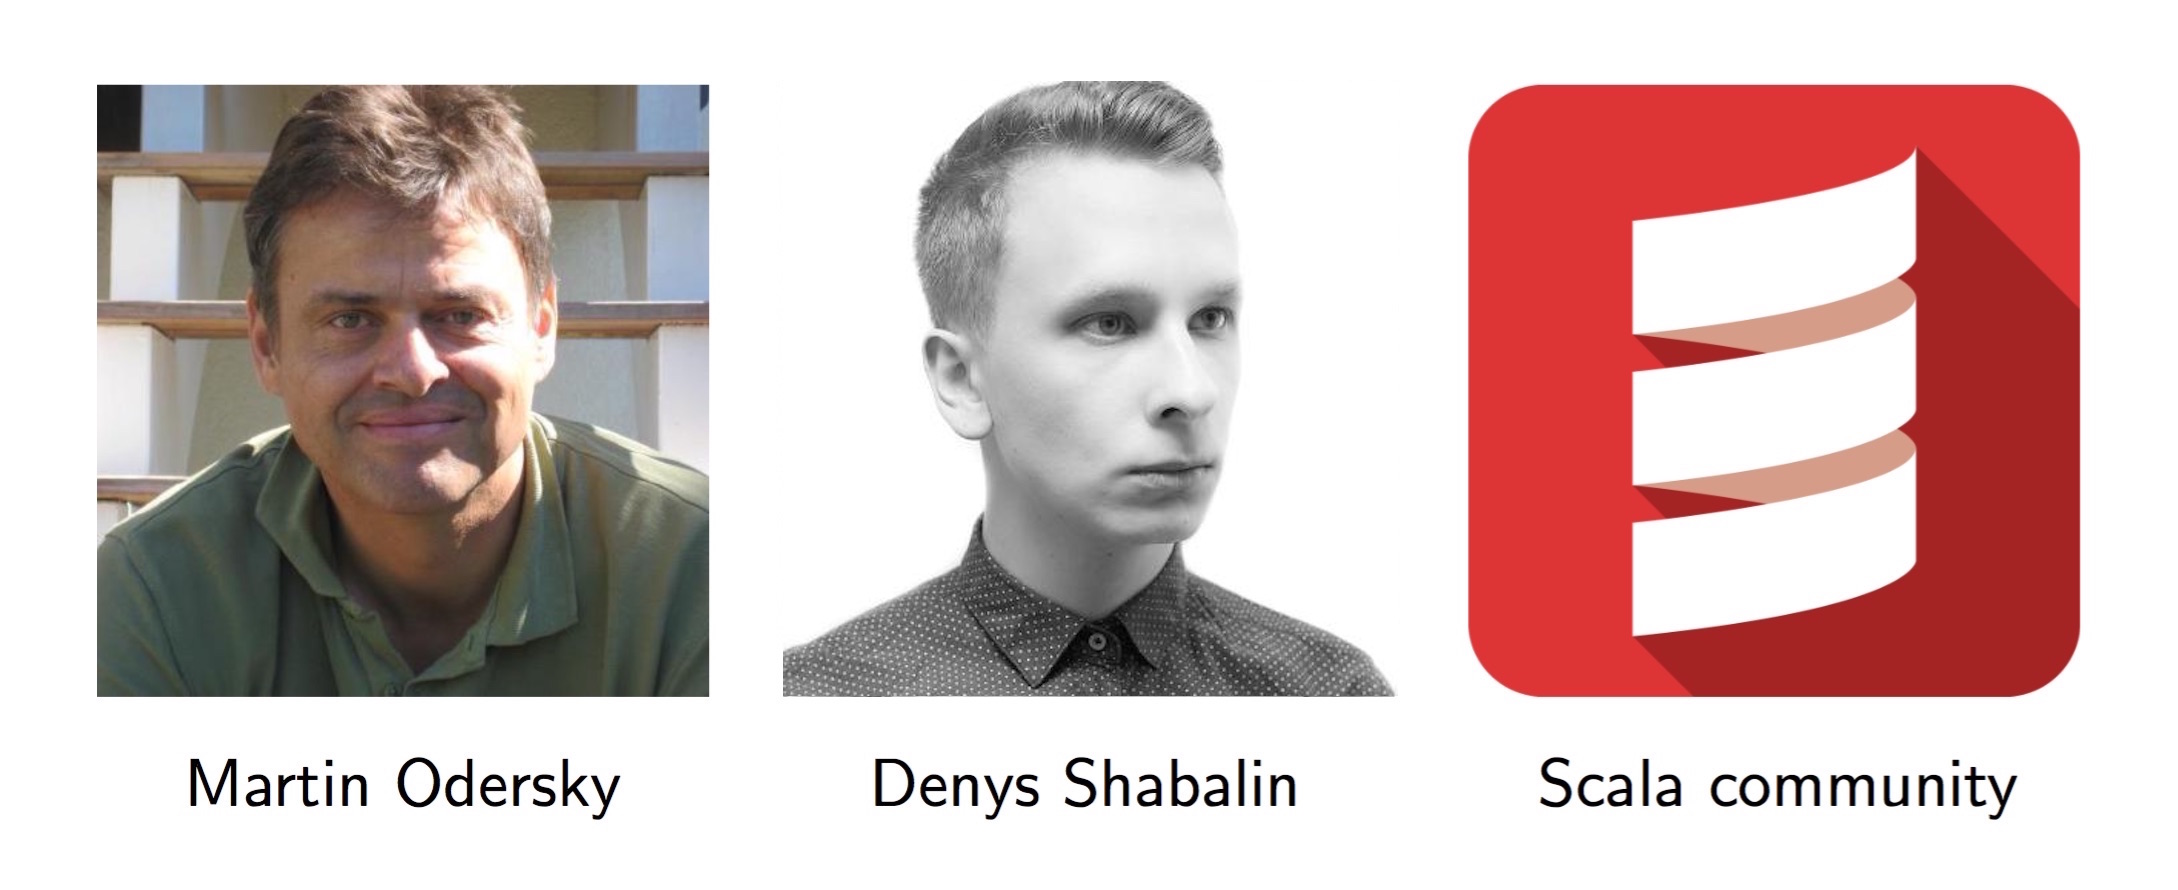
\includegraphics[height=5cm]{credits.jpeg}
\end{frame}

\begin{frame}{Summary}
\begin{itemize}
\item Scala macros are a powerful and popular language feature
\item Their best part is the combination of metaprogramming and types
that makes it possible to enrich existing language features
\item Their worst part is the ad hoc metaprogramming API
that significantly raises the barrier to entry and complicates tool support
\item A better metaprogramming API that initially targeted macros 2.0
ended up being useful on its own for development of novel tools.
\end{itemize}
\end{frame}

\end{document}